

\chapter{Future Work}\label{C:Future Work}

Going forward it will be important to move from working with two bit images back up to larger images with non-toy models - i.e. the MNIST handwritten digit dataset.
An outcome of the next step is being able to train two RBMs from purely composite data. For instance, being able to train an RBM that learnt a representation of a digit and another of noise from only seeing digits combined with noise. If this is fruitful, it will amount to blind source separation.

It is worth noting that out of scope at the moment is using actual photos, as this would require significantly more computing power. The runtime of this new approach needs to be tested for correctness on smaller images before this can occur. Also this might require aligning the content images and potentially acquiring a larger image dataset. Working with datasets like MNIST where this has already been applied allows the focus to be on evaluating the new technique.

\begin{figure}
  \begin{center}
    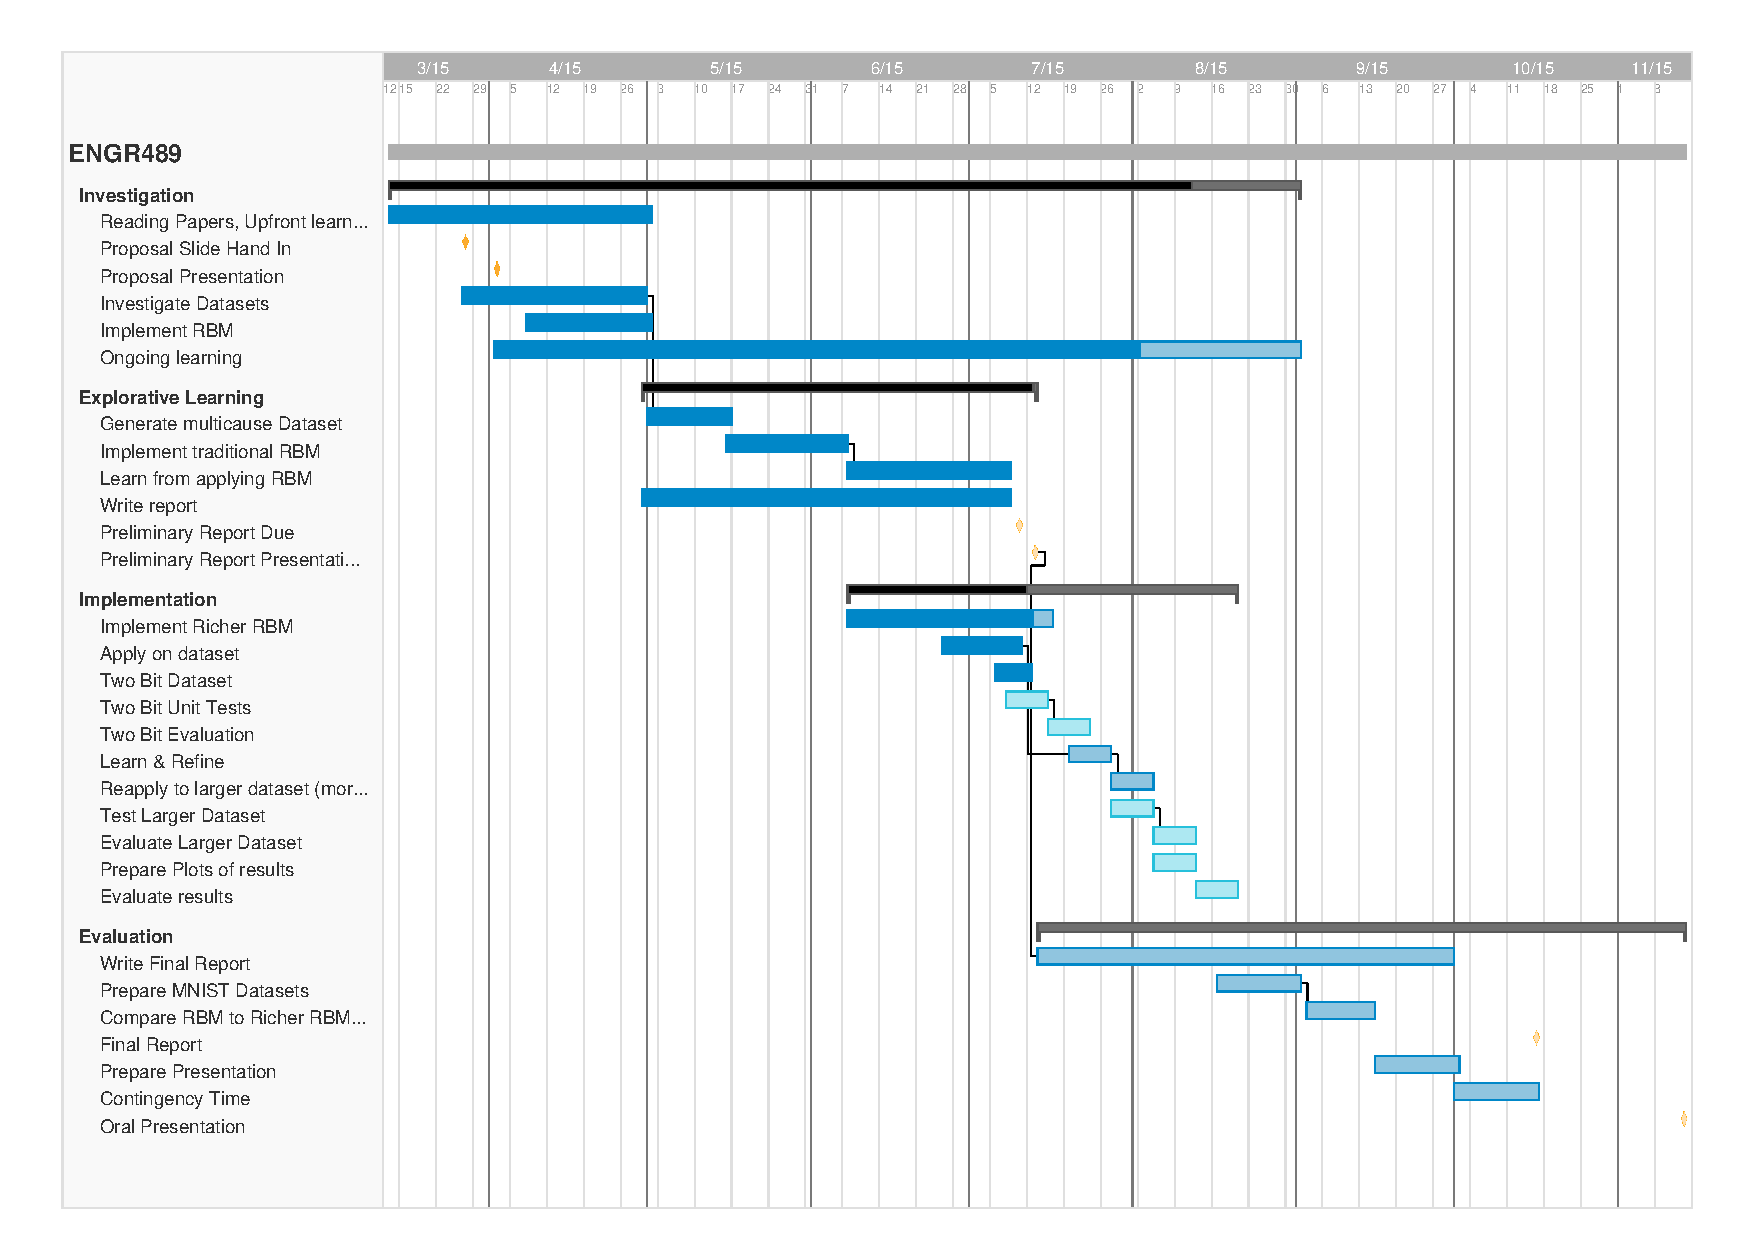
\includegraphics[width=1\textwidth]{Assets/gantt}
    \caption{Revised Gantt chart}
   \label{F:gantt}
   \end{center}
\end{figure}





